\documentclass[10pt]{article}

\usepackage{amsfonts, amsthm, amsmath, fullpage, tikz, wrapfig, enumerate}

\newcommand{\card}[1]{\left| #1 \right|}
\newcommand{\brackets}[1]{\left< #1 \right>}
\newcommand{\nat}{\mathbb{N}}
\newcommand{\ints}{\mathbb{Z}}
\newcommand{\reals}{\mathbb{R}}
\newcommand{\chtitle}[1]{\noindent \vspace{5mm}\textbf{Chapter #1}\vspace{3mm}}

\begin{document}
\begin{flushleft}
\textbf{\noindent
CS 341 Automata Theory \\
STUDENT NAME - EID\\
Homework 13 \\
Due: Tuesday, April 17}\\
\end{flushleft}

\noindent
This assignment covers Sections 21.1 - 21.3\\

\begin{enumerate}[1)]

% ---
% 1
% ---

\item
In Appendix E.3, we describe a straightforward use of reduction that solves a grid coloring problem by reducing it to a graph problem.  Given the grid $G$ shown here:
\begin{center}
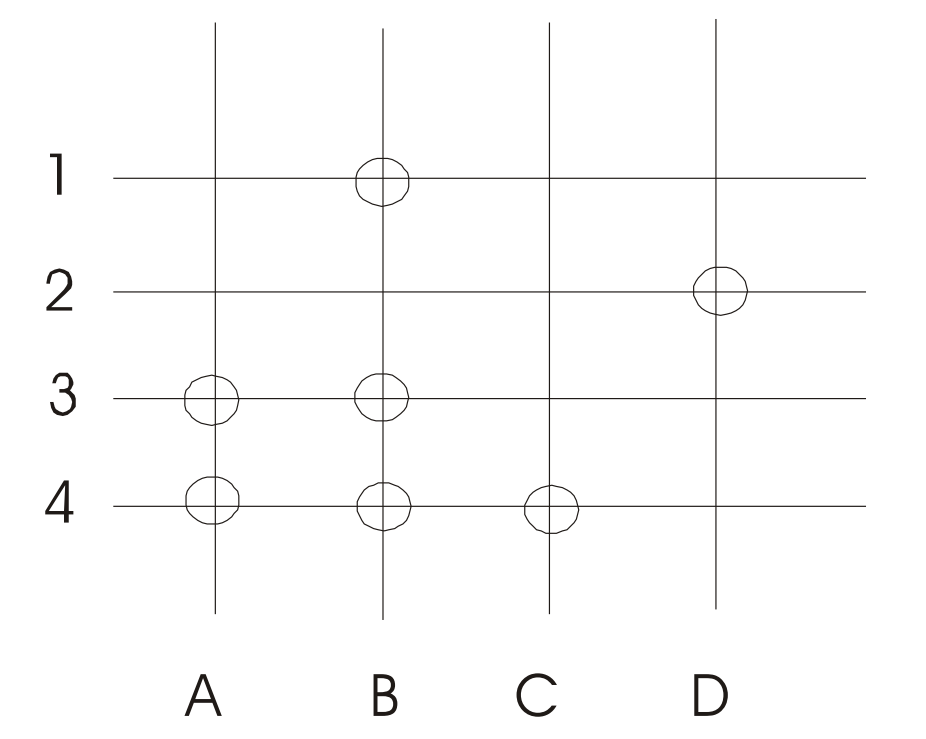
\includegraphics[scale=.15]{images/p1.png}
\end{center}
\begin{enumerate}[a)]

%a
\item
Show the graph that corresponds to $G$.
\begin{proof}[Solution]
\end{proof}

%b
\item
Use the graph algorithm we describe to find a coloring of $G$.
\begin{proof}[Solution]
\end{proof}
\end{enumerate}


%---
% 2
%---

\item
In this problem, we consider the relationship between $H$ and a very simple language $\{a\}$.
\begin{enumerate}[a)]

%a
\item
Show that $\{\texttt{a}\}$ is mapping reducible to $H$.  
\begin{proof}[Solution]
\end{proof}

%b
\item
Is it possible to reduce $H$ to $\{\texttt{a}\}$?  Prove your answer.
\begin{proof}[Answer]
\end{proof}
\begin{proof}[Proof]
\end{proof}
\end{enumerate}

% ---
% 3
% ---

\item
Show that $H_{ALL}$ is not in $D$ by reduction from $H$.
\begin{proof}[Solution]
\end{proof}


% ---
% 4
% ---

\item
For each of the following languages $L$, state whether or not it is in $D$.  Prove your answer.  Assume that any input of the form $\brackets{M}$ is a description of a Turing machine.
\begin{enumerate}[a)]

%a
\item
$\{\brackets{M}\ :\ \texttt{ab} \in L(M)\}$.
\begin{proof}[Answer]
\end{proof}
\begin{proof}[Proof]
\end{proof}

%b
\item
$\{\brackets{M, w}$ : TM $M$, on input $w$, begins by moving right one square onto $w$.  Then it never moves off $w$\}.
\begin{proof}[Answer]
\end{proof}
\begin{proof}[Proof]
\end{proof}

%c
\item
$\{\brackets{M}$ : there exists a string $w$ such that $\card{w} < \card{\brackets{M}}$ and that $M$ accepts $w$\}.
\begin{proof}[Answer]
\end{proof}
\begin{proof}[Proof]
\end{proof}
\end{enumerate}

% ---
% 5
% ---

\item
In Appendix J.2, we proved Theorem J.1, which tells us that the safety of even a very simple security model is undecidable, by reduction from $H_\epsilon$.  Show an alternative proof that reduces $A = \{\brackets{M, w}$ :  $M$ is a Turing machine and $w \in L(M)$\} to the language Safety.
\begin{proof}[Proof]
\end{proof}
\end{enumerate}
\end{document}
